\chapter{Proposed System Architecture}

% I'm thinking this could be a bit like a whitepaper, where I outline the requirements for the Ahuora Digital Twin Platform, and how I think it should be implemented.
% then the other sections can go into more depth, to confirm my argument that this is the best way to implement the platform.

% Digital Twin Software needs to suit the use cases of Network Administrators, Chemical Engineers, Process Engineers, and Operators to be useful in industry.
% Steady-State, Dynamic, and Surrogate modelling are all required to support the different use cases.
% A Digital Twin platform needs to integrate with existing SCADA systems and data processing tools to be useful in industry.

% Simulation results need to be avalible within the platform, but this should not replace the company's existing knowledge base/data lake/logging.
% There is no need for Ahuora to develop a new data processing platform, as SCADA systems or things such as kafka/mqtt do this fine.
% It should be easy to switch between design and operation modes, assuming the network administrator has set up the external data processing platform/sources.
% The Ahuora Digital Twin Platform needs to be designed to support these requirements.

% What Hypothesis am I testing here?
% How do I recommend that the above be implemented?



Conventional simulation platforms do not have built-in support for live data processing. Likewise, conventional factory SCADA\footnote{SCADA systems: Supervisory Data Aquisition and Control systems.} systems do not have built-in support for complex simulation. To integrate a simulation platform with live data, a software system must be created that can merge the two systems. This can be considered as an intermediate layer between the simulation platform and the factory SCADA system.


\begin{figure}[h]
    \centering
    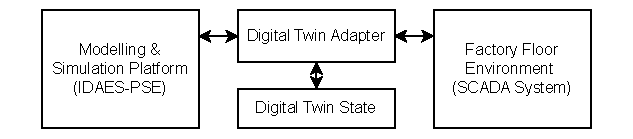
\includegraphics[width=0.8\textwidth]{research_article/research_journal_framework_simple.pdf}
    \caption{Theoretical framework of how a Digital Twin can be implementend on top of existing simulators and factory control systems.}
    \label{fig:theoretical_framework}
\end{figure}

The concept of a “Digital Twin” refers to a simulation of something in the physical world, which is kept up to date with a physical system using real-time data \cite{yu2022energy}.
In \cref{fig:theoretical_framework}, this intermediate layer is what converts the simulation platform, and the data from the factory, into a digital twin. 

By breaking the Digital Twin up into these core components, we are able to make use of existing software systems for live data processing and simulation, and only need to build the components that are unique to the Digital Twin use case. This limits the complexity of the system, and means that implementing a Digital Twin in a factory can be done with minimal disruption to the existing systems.

% These sections should be presenting the arguments that we will make in all the other sections.

\section{Modelling and Simulation Platform}


Being able to model and simulate a process is one of the foundational components of a Digital Twin platform. 

Conventionally, simulation platforms are used when designing and planning a factory, and are not used during operation. This makes most conventional simulation platforms unsuitable for use in a Digital Twin, without substantial modification.
In the Ahuora Platform, IDAES-PSE provides the core modelling and simulation capabilities. 
It is built on top of Pyomo, an Algebraic Modelling Language, enabling for flexible model definitions.
This flexibility is key in enabling a Digital Twin platform to be built on top of IDAES. 
Further flexibility is enabled through the Ahuora Platform, which can be modified to support whatever features are required.

% Todo: Give Examples, link to sections that go through the different parts
\section{Factory Floor Environment}

In the factory, there are many sensors and control systems that monitor the state of the factory. These systems are often connected to a SCADA system, which is responsible for collecting and displaying this data.
Additionally, there are often data processing systems that are used to store and process this data, as historical data is often used in later analysis to improve performance or make maintenance and upgrade decisions.

There are also automated and manual control systems, which are used to adjust the factory's operation based on the data collected by the SCADA system.
These systems are already implemented in factories, and are critical to the operation of the factory.

% Todo: Give Examples, link to other sections
\section{Digital Twin Adapter}

As such, rather than making a new data processing system, it is better that a Digital Twin Platform can be built such that it can be implemented on top of established data processing systems. Likewise, rather than making a new simulation platform, it is better if the framework of an existing simulation platform can be reused or adapted to the digital twin use case.

The concept of a ``Digital Twin Adapter'' is used to define this functionality. It is responsible for converting the data from the factory into a format that the simulation platform can understand, and to provide results from simulations back the factory.


% Todo: give examples, link to other sections
\section{Digital Twin State}

Key to the sucessful operation of the the Digital Twin Adapter is the fact that is also has access to the ``Digital Twin State". The Digital Twin State represents an estimate of the current state of the factory, based on the simulation results and the live data. 
This represents the ability of a Digital Twin to "learn" how the physical system behaves, and adjust the inputs to the simulation accordingly.


% Todo: Give examples, link to other sections.

\section{Limitations of the Proposed Architecture}

This architecture generalises the concept of a Digital Twin, enabling software to be built that can be used in a wider variety of factories. However, the exact implementation of the Digital Twin Adapter may need to change depending on the factory's existing systems. Different SCADA systems and data processing systems will have different ways of communicating, and different data will be avaliable depending of the factory. Likewise, different methods of simulation may or may not be avaliable depending on the system. 

The Digital Twin Adapter will need to be built in a way that it can be customised or set up differently depending on the factory. 
